\documentclass[a4paper,10pt]{article}

\usepackage[utf8]{inputenc} 
\usepackage[T1]{fontenc}     
\usepackage[francais]{babel}

\usepackage[top=2cm, bottom=2cm, left=2cm, right=2cm]{geometry}

\usepackage{graphicx}

\usepackage{amsthm}
\usepackage{amsmath}
\usepackage{amssymb} 	

\usepackage{url}

\usepackage{algorithm}
\usepackage{algorithmic}
%\usepackage[backref, hidelinks]{hyperref}

\usepackage{a4wide}

%%%% debut macro %%%%
\newenvironment{changemargin}[3]{\begin{list}{}{%
\setlength{\topsep}{0pt}%
\setlength{\leftmargin}{0pt}%
\setlength{\rightmargin}{0pt}%
\setlength{\topmargin}{0pt}%
\setlength{\listparindent}{\parindent}%
\setlength{\itemindent}{\parindent}%
\setlength{\parsep}{0pt plus 1pt}%
\addtolength{\leftmargin}{#1}%
\addtolength{\rightmargin}{#2}%
\addtolength{\topmargin}{#3}%
}\item }{\end{list}}
%%%% fin macro %%%%


\title{{\huge Présentation de l'article :} \\
Interactive Control of Diverse Complex Characters with Neural Network \cite{NIPS2015_5764}}
\author{\textsc{Kozolinsky} Jules}
\date\today 
\makeindex

\begin{document}

\maketitle
\tableofcontents

\section{Introduction}
\subsection{Contexte}
  Présenté lors de la conférence d'intelligence artificielle NIPS 2015, cet article écrit par les chercheurs, Igor Mordatch, Kendall Lowrey, Galen Andrew, Zoran Popovic et Emanuel Todorov, de l'université de Washington propose une méthode capable d'entrainer un réseau de neurones à se comporter comme une politique dotée d'un feedback quasi optimal. 

\subsection{Objectif de l'article}
  On souhaite que la politique issue du réseau de neurones entrainé s'applique à tout type d'entités et de morphologies, soit capable d'opérer en temps réel et soit insensible au bruit pouvant exister. Elle est appliquée ici à des tâches de déplacement (nage, vol, marche bipède et quadrupèdes pour différentes morphologies). La méthode utilisée s'appuie principalement sur l'optimisation de trajectoires avec du bruit et l'apprentissage supervisé d'un réseau de neurones. 

%\subsection{Les difficultés du problèmes}

\section{Principe global}
La méthode consiste à apprendre au réseau de neurones à générer des trajectoires similaires à celle de l'optimiseur hors ligne.
\subsection{Définitions}
\paragraph{Etat de l'entité} On définit l'état d'une entité comme la matrice $(q~f~r)$ où $q$ est l'état physique, (par exemple la position, l'orientation, l'angle des joints, ...), $f$ sont les forces de contact avec le sol et $r$ est la mémoire (non définie dans l'article, mais permettant sûrement de stocker des informations numériquement utile pendant la trajectoire).
\paragraph{Trajectoire} La trajectoire de l'entité est la succession d'états pendant une période $T$ : 
\[ X = (q^0~f^0~r^0~...~q^T~f^T~r^T) \]
\paragraph{Politique issue du réseau de neurones\\}
La politique est une fonction :
\[ \pi_{\theta} : s \mapsto a \] où 
\begin{itemize}
\item $\theta$ est le vecteur des poids du réseau de neurones,
\item $s^t(X) = (q^t~r^t~\dot{q}^{t-1}~f^{t-1})$  est \textit{l'état sensoriel} au temps $t$ de la trajectoire $X$,
\item $a^t(X) = (\dot{q}^{t}~\dot{r}^{t}~f^{t})$ est \textit{l'action optimale} au temps $t$ de la même trajectoire $X$.
\end{itemize}
(On a noté $\dot{x}^t = x^{t+1}-x^t$, proche de la dérivée temporelle de $x$ pour $\Delta t$ petit).\\
\textbf{Note :} On peut remarquer en observant l'expression de l'action optimale que le réseau de neurones apprends non seulement le contrôle optimal mais aussi le modèle dynamique sous-jacent. 
\subsection{Description du problème}
L'objectif se réduit au problème d'optimisation sous contrainte égalité suivant : 
  \begin{align}
  \min_{\theta,X^1,...,X^N} \sum\limits_{i=1}^{N} C_{i}(X^{i}) \hspace{15pt}\text{ \small sachant } \hspace{5pt} \forall i,t : a^{t}(X^{i}) = \pi_{\theta}(s^{t}(X^{i}))
  \end{align}
où
  \begin{itemize}
  \item $\theta$ est le vecteur des poids du réseau de neurones (qui sera utilisé pour exécuter la politique en temps réel après optimisation)
  \item $X^{i}$ trajectoire d'objectif $i$ (on prends différentes conditions initiales pour les différentes tâches)
  \item $C(X)$ est le coût total de la trajectoire $X$ (explicité plus tard).
  \end{itemize}
  
\subsection{Trajectoire bruitée}
On ne va pas calculer uniquement les trajectoires optimales mais aussi les mêmes trajectoires \textit{entourées} de bruits, \textit{i.e.} ajouter du bruit à l'état sensoriel, en entrée de la politique. 
\subsubsection{L'intérêt du bruit}
D'après d'autres articles, ajouter du bruit lors de l'entrainement du réseau de neurones produits des mouvements plus robustes \cite{huh2009real} \cite{wang2010optimizing}. La politique est en effet capable de se corriger et de tendre alors vers la trajectoire optimale (sans bruit). D'autre part, ajouter du bruit réduit le sur-apprentissage \cite{hinton2012improving} et stabilise le comportement du réseau de neurones \cite{hoerzer2014emergence}. Ici on ajoute principalement du bruit pour éviter que la politique diverge lors de son exécution en temps réel. 

\subsubsection{L'ajout du bruit}
On ajoute donc un bruit gaussien $\varepsilon \sim \mathcal{N}(0,\sigma_{\varepsilon}^{2}I)$ (où $\sigma_{\varepsilon}^{2} \simeq 10^{-2}$) dans l'expression de la politique : 
\begin{align*}
  \pi_{\theta}(s + \varepsilon) = a + a_{s}\varepsilon 
\end{align*}
où $a_s$ est le gradient lors du développement limité au premier ordre. Cette matrice représente le feedback optimal autour de l'état sensoriel $s$. Nous verrons dans la partie suivante pour son calcul explicite. ($a$ sera quant à lui calculer par optimisation de la trajectoire $X$)

\subsection{Algorithme}
 Reprenons le problème d'optimisation avec contraintes égalités en ajoutant ce bruit gaussien. Ce problème n'étant pas convexe, on remplace cette contrainte \textit{dure} par une pénalité quadratique : 
 \begin{align*}
  \min_{\theta,X^1,...,X^N} \sum\limits_{i=1}^{N} C_{i}(X^{i}) + \sum\limits_{i,t} R(s^{t}(X^{i}),a^{t}(X^{i}),\theta,\varepsilon^{i,t})\\ \text{\footnotesize avec } \hspace{5pt}
  R(s,a,\theta,\epsilon) = \frac{\alpha}{2}||(a+a_s\varepsilon) - \pi_{\theta}(s+\epsilon)||^2
  \end{align*}
où $\alpha$ est la pénalité quadratique. ($\alpha \simeq 10$.)\\


Cela mène à l'algorithme suivant : 
\begin{algorithm}
\caption{}
\begin{algorithmic}
\STATE $1.$ Échantillonner le bruit $\varepsilon^{i,t}$
\STATE $2.$ Optimiser $N$ trajectoires indépendamment : 
\begin{align*}
\forall i, \hspace{3pt} \bar{X}^{i} = \text{argmin}_{X} ~C_{i}(X) + \sum_{t} R(s^t(X),a^t(X),\bar{\theta},\bar{\varepsilon}^{i,t}) + \frac{\eta}{2}||X-\bar{X}^{i}||^2
\end{align*}
\STATE $3.$ Entrainer le réseau de neurones (régression) : 
\begin{align*}
\bar{\theta} = \text{argmin}_{\theta} ~\sum_{i,t} R(s^t(\bar{X}_i),a^t(\bar{X}_i),\theta,\bar{\varepsilon}^{i,t}) + \frac{\eta}{2}||\theta-\bar{\theta}||^2
\end{align*}
\STATE $4.$ Répéter
\end{algorithmic}
\end{algorithm}
\\
\textbf{Note : } On a ajouté un terme de régularisation de paramètre $\eta \simeq 10^{-2}$.

\section{Optimisation de trajectoire}
Détaillons dans cette section la deuxième étape de l'algorithme. On souhaite trouver une trajectoire optimale débutant d'une certaine condition initiale et réalisant une tâche tout en vérifiant la réalité physique, \textit{i.e.} les équations de la dynamique. 
(La partie d'optimisation de trajectoire simple (sans bruit) est basé sur \textit{Discovery of Complex Behaviors through Contact-Invariant Optimization} \cite{mordatch2012discovery} impliquant une partie des chercheurs travaillant sur cet article.)
\subsection{Vérifier les équations de la dynamique}
Les paramètres doivent vérifier les équations de la dynamique suivantes : 
\begin{align*}
H(q)\ddot{q} + \hat{C}(q,\dot{q}) = \tau + J(q,\dot{q})^{\top}f, \hspace{15pt}
 d(q) \geq 0,  \hspace{10pt}
 d(q)^{\top}f = 0,  \hspace{10pt}
 f \in K(q) 
  \end{align*}
où
  \begin{itemize}
  \item $f$ forces de contacts sur les organes terminaux
  \item $\tau$ inverse de la dynamique
  \item $H$ matrice d'inertie
  \item $\hat{C}$ matrice de Coriolis et des forces centrifuges
  \item $J$ matrice Jacobienne
  \item $d(q)$ distance au sol
  \item $K(q)$ cône de friction
  \end{itemize}
\paragraph{}
  
  Ces contraintes sont ajoutées avec un terme de pénalité dans le coût total $C(X)$. (On fait de même avec les conditions initiales.)
  
\subsection{Calcul de la trajectoire optimale}
\subsubsection{Définition du coût total}
Définissons le coût total de la manière suivante : 
  \begin{align*}
  C(X) = \sum\limits_{t}c^t(\phi^t(X))
  \end{align*}
où 
  \begin{itemize}
  \item $\phi^t(X)$ extrait les caractéristiques nécessaires pour calculer le coût de la trajectoire $X$
  \item $c(\phi)$ coût à partir de ces caractéristiques de la trajectoire
\end{itemize} 
\paragraph{}
Pour simplifier, on écrit le problème d'optimisation précédant sous la forme suivante (on mets tous les objectifs \textit{à l'intérieur} de $C$): 
  \begin{align*}
  X^* = \text{argmin}_{X} C(X)
  \end{align*}
\subsubsection{Méthode de Quasi-Newton}
On utilise la méthode de quasi-Newton pour résoudre ce problème d'optimisation. $D^2_{X}$ est ainsi calculé par approximation de Gauss-Newton. D'autre part, $c$ est choisi tel que son gradient et sa Hessienne soit calculable analytiquement, alors que $\phi$ est calculé par différence finie.
Ainsi la trajectoire optimale vérifie l'équation suivante : 
  \[
  X^{*} = X^{*} - D^2_{X}C(X)^{-1}\nabla_{X}C(X) 
  \]
  \textbf{Note :} On ne lance pas cet algorithme jusqu'à convergence de $X^{*}$ mais on ne fait que quelques itérations (entre $1$ et $10$).
 \subsection{Calcul de la trajectoire optimale bruitée}
  On souhaite calculer la trajectoire optimale bruitée $\tilde{X}$, perturbation de la trajectoire optimale $X$ telle que $s(\tilde{X}) = \bar{s} = s + \varepsilon$. \\
  Le bruit intervient dans l'expression de la politique développée au premier ordre : 
  \[ \pi_{\theta}(s(\tilde{X})) = \pi_{\theta}(s + \varepsilon) = a + a_{s}\varepsilon = a(\tilde{X}) \]. 
  \subsubsection{Calcul de la matrice de feedback optimale $a_{s}$}
  L'action optimale $a$ a été calculée lors du calcul de la trajectoire optimale $X$. Il suffit donc de calculer la matrice de feedback optimal $a_{s}$.
  Par une règle de gradient composé, on obtient : 
  \[
  a_{\bar{s}} = a_{X}\tilde{X}_{\bar{s}}
  \]
  Or le gradient de $a$ par rapport à $X$ a déjà été calculé lors du calcul de $\phi_X$, car les fonctions $a$ et $\phi$ sont des fonctions qui extraient les caractéristiques de la trajectoire $X$. (Il en va de même pour $s_X$.)
  \subsubsection{Calcul du gradient $\tilde{X}_{\bar{s}}$}
  La trajectoire optimale bruitée est solution du problème d'optimisation suivant : 
  \[
  \tilde{X}(\bar{s}) = \text{argmin}_{X^{*}} \big{(}C(X^{*}) + \frac{\lambda}{2}||s(X^{*}) - \bar{s}||^{2}\big{)}
  \]
  Ainsi, par approximation à partir de la trajectoire optimale non bruitée et de la méthode de Quasi-Newton (où $\lambda \simeq 10^2$),
  \[
  \tilde{X}(\bar{s}) = X - (C_{XX} + \lambda s_{X}^{\top}s_{X})^{-1}(C_{X} + \lambda s_{X}^{\top}(s(X) - \bar{s})
  \]
  Dont le gradient est : 
    \[
  \tilde{X}_{\bar{s}} = \lambda(C_{XX} + \lambda s_{X}^{\top}s_{X})^{-1}s_{X}^{\top}
  \]
  dont on a déjà calculé l'ensemble des termes.
  
\section{Entrainement du réseau de neurones}
\subsection{Utilisation du réseau de neurones}
\paragraph{}
Passons à l'étape suivante de l'algorithme. On souhaite entrainer le réseau de neurones, \textit{i.e.} effectuer une régression. En effet, on a les données d'entrainement $(s + \varepsilon, a + a_{s}\varepsilon)^{i,t}$ (calculées lors de l'étape précédentes) et on souhaite calculer $\theta$ le vecteur des poids du réseau de neurones apparaissant dans la politique $\pi_{\theta} : s \mapsto a$.
\paragraph{}
L'article ne détaille que très peu le fonctionnement des réseaux de neurones, utilisés comme une boîte noire d'optimisation, là où nous aurions pu utiliser d'autres méthodes d'apprentissage supervisé pour les régressions. 
\subsection{Paramètres du réseau de neurones}
Le réseau de neurones est donc constitué, en plus des couches d'entrée et de sortie, de trois couches cachées, chacune possédant 250 neurones. La fonction d'activation est une fonction classique des réseaux de neurones : $\tanh$. Ces paramètres ont été choisis grâce au compromis complexité/erreur suivant : \\
\begin{center}
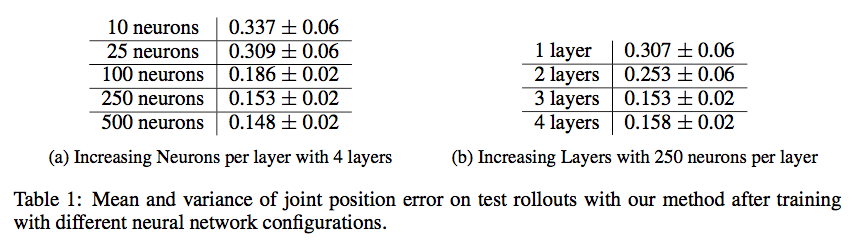
\includegraphics[scale=0.4]{nn}
\end{center}

\section{Exécution de la politique}
A présent, l'algorithme hors-ligne a été détaillé et lorsqu'il termine, nous obtenons un réseau de neurones entrainé agissant comme une politique $\pi_{\theta^{*}} : s \mapsto a$.\\
En robotique, on appliquerait cette politique sur le robot et cela déterminerait les forces à appliquer à chacun des moteurs. \\
En animation, on souhaite calculer la position suivante de l'entité. Pour cela un simple problème d'optimisation à horizon $T=1$ suffit. 

\section{Résultats}
Pour les expériences, un pas de temps de $\Delta t = 50$ ms a été utilisé. Les résultats des expériences sont présentés dans la vidéo suivante. Il a été demandé à des entités de morphologies différentes de nager, voler et de marcher. \\
 Video : \url{https://www.youtube.com/watch?v=IxrnT0JOs4o}
 Le comportement cyclique lors du vol est assez impressionnant car il n'a été codé nulle part. Celui-ci découle simplement de l'optimisation faite lors de l'algorithme. Il en va de même pour la marche où les pas droite-gauche n'ont pas été directement implémentés dans l'interface. L'entité lève les pieds, car conformément à l'article \textit{Discovery of Complex Behaviors through Contact-Invariant Optimization} \cite{mordatch2012discovery}, le glissement n'est pas autorisé. 
\section{Conclusion}
\paragraph{}
Finalement cette algorithme comportant une phase hors-ligne d'optimisation et d'apprentissage supervisé, pour obtenir un réseau de neurones entrainé se comportant comme une politique,  semble très efficace, d'autant plus qu'il se déploie en temps réel. 
Cet article va dans le sens où on souhaite trouver des politiques en temps réel pour les appliquer sur les robots. 
\paragraph{}
Dans l'article, seulement des tâches de déplacement ont été implémentés. On pourrait s'intéresser à d'autres tâches moins triviales tels escalader, se relever ou encore ouvrir une porte.\\
D'autre part, on pourrait utiliser d'autres algorithmes d'apprentissage que les réseaux de neurones. 


\bibliographystyle{plain}
\bibliography{biblio}


\end{document}
